\section{Introducción}

El problema de encontrar la subsecuencia de suma máxima consiste en determinar, dentro de un arreglo de números enteros, 
la subsecuencia contigua cuya suma de elementos sea la mayor posible. Este problema es clásico en el análisis de algoritmos, 
ya que permite comparar distintas estrategias de solución y analizar su complejidad computacional.

Para esto se implementaron en C++ cuatro algoritmos discutidos en clase para resolver el problema de la subsecuencia de suma máxima.
Cada uno de estos algoritmos presenta una complejidad temporal distinta, lo que permite observar cómo el diseño algorítmico influye 
directamente en el tiempo de ejecución al aumentar el tamaño de la instancia.

Una vez verificado el funcionamiento correcto de las implementaciones, se realizaron experimentos para medir los tiempos de ejecución 
utilizando arreglos de diferentes tamaños. Las pruebas se llevaron a cabo para valores crecientes de $n$, comenzando desde $n=10$ y 
aumentando progresivamente hasta tamaños mayores, manteniendo siempre la misma instancia de datos para todos los algoritmos con el 
fin de garantizar una comparación justa de los tiempos de ejecución.

Además de los cuatro algoritmos presentados en clase, se propuso un algoritmo adicional cuya eficiencia es al menos equivalente al 
mejor de los algoritmos analizados. 

\subsection{Caracteristicas Computacionales}

El equipo propio donde se corrieron los experimentos cuenta con las siguientes características computacionales:

\begin{figure}[H]
    \centering
    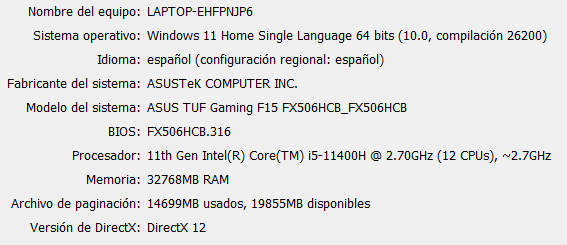
\includegraphics[width=0.5\textwidth]{rsc/img/pc_dg.png}
    \caption{Características computacionales del equipo utilizado para los experimentos.}\label{fig:comp}
\end{figure}

Mientras el equipo de la supercomputadora LAVIS cuenta con las siguientes características computacionales:

\begin{itemize}
    \item 6 nodos de computo con 186 procesadores en todos los nodos en conjunto.
    \item Procesador:  Intel (R) Xeon (R) E3--1230 (3.50GHz)
    \item Memoria RAM (Nodo): 16 GB de RAM
    \item Sistema operativo: Rocky Linux
    \item Lenguaje de programación: C++
\end{itemize}